\documentclass[14pt,a4paper]{extarticle}

\usepackage{fontspec}
\usepackage{babel}
\babelprovide[import,main]{russian}
\usepackage{geometry}
\usepackage{graphicx}
\usepackage{indentfirst}
\usepackage{hyperref}

\setmainfont{Times New Roman}[
  Path=/System/Library/Fonts/Supplemental/,
  UprightFont=Times New Roman.ttf,
  BoldFont=Times New Roman Bold.ttf,
  ItalicFont=Times New Roman Italic.ttf,
  BoldItalicFont=Times New Roman Bold Italic.ttf
]

\geometry{left=2.5cm,right=1.5cm,top=2cm,bottom=2cm}
\setlength{\parindent}{1.25cm}
\setlength{\emergencystretch}{3em}
\hfuzz=6pt
\linespread{1.08}
\pagestyle{empty}
\hypersetup{
  colorlinks=true,
  urlcolor=blue,
  pdftitle={Работа №1. Разработка защищённого REST API с интеграцией в CI/CD},
  pdfauthor={Перминов Юрий Константинович},
  pdfsubject={Информационная безопасность}
}

\newcommand{\head}[1]{%
  \par\vspace{0.9em}%
  \noindent\textbf{#1}\par\vspace{0.35em}%
}

\begin{document}

\begin{titlepage}
\centering
Федеральное государственное автономное\\
образовательное учреждение высшего образования\\
«Национальный исследовательский университет ИТМО»

\vspace{3.2cm}
\textbf{Информационная безопасность}

\vspace{0.9cm}
\textbf{Работа №1}\\[0.35em]
«Разработка защищённого REST API с интеграцией в CI/CD»

\vspace{3.4cm}
\begin{flushright}
Выполнил: Перминов Юрий Константинович\\
Группа: P3431\\
Практик: Рыбаков Степан Дмитриевич
\end{flushright}

\vfill
2026
\end{titlepage}

\head{Выполнение}

\noindent\textbf{Ссылка на GitHub репозиторий}\\
\url{https://github.com/tinunadno/ib-lab1.git}

\head{Описание проекта}

Небольшой сервис на Flask: вход по логину и паролю, выдача JWT и доступ к данным только с валидным токеном. Аутентифицированный пользователь получает список пользователей и может сохранить сообщение. На каждый push и pull request в ветку develop GitHub Actions прогоняет тесты, статический анализ кода (SAST) и проверку зависимостей (SCA).

\head{Стек}

\begin{itemize}
  \item Python 3.12, Flask
  \item SQLite (файл \texttt{app.db})
  \item PyJWT --- токены, bcrypt --- хеширование паролей, \texttt{html.escape} --- экранирование вывода
  \item bandit (SAST) и pip-audit (SCA) в CI
\end{itemize}

\head{Описание API}

\begin{center}
\renewcommand{\arraystretch}{1.25}
\begin{tabular}{|l|l|l|p{5.6cm}|}
\hline
Метод & Путь & Доступ & Описание \\
\hline
POST & \texttt{/auth/login} & все & вход, возвращает JWT \\
\hline
GET & \texttt{/api/data} & по токену & список пользователей \\
\hline
POST & \texttt{/api/messages} & по токену & сохранить сообщение \\
\hline
\end{tabular}
\end{center}

Неверная пара логин/пароль --- 401. Без токена или с невалидным токеном запросы к \texttt{/api/data} и \texttt{/api/messages} возвращают 401. Пустой текст сообщения --- 400.

\head{Реализованные меры защиты}

\textbf{SQL-инъекции}

Все запросы к базе параметризованные: в SQL стоят плейсхолдеры \texttt{?}, значения передаются отдельным аргументом, строки не склеиваются:

\begin{quote}
\begin{verbatim}
db().execute(
    "select id, password from users where username = ?",
    (username,),
)
\end{verbatim}
\end{quote}

Драйвер SQLite подставляет значение как данные, а не как часть запроса, поэтому ввод вида \texttt{' OR 1=1 --} просто ищется как логин и ничего не находит.

\textbf{XSS}

Пользовательские строки в ответах (имя пользователя и текст сообщения) проходят через \texttt{html.escape} перед выдачей. Тег \texttt{<script>} возвращается как \texttt{\&lt;script\&gt;} и в браузере не выполняется.

\textbf{Аутентификация}

\begin{itemize}
  \item Пароли хешируются bcrypt со случайной солью, в базе только хеш. bcrypt намеренно медленный, поэтому перебор по украденной базе дорогой.
  \item JWT. После входа выдаётся токен HS256 с id пользователя (\texttt{sub}) и сроком действия (1 час). Секрет подписи берётся из переменной окружения \texttt{JWT\_SECRET}, в коде его нет.
  \item Проверка токена. Декоратор \texttt{auth} стоит на \texttt{/api/data} и \texttt{/api/messages}: проверяет заголовок \texttt{Authorization: Bearer}, подпись и срок действия; разрешён только алгоритм HS256, поэтому токен с \texttt{alg: none} не пройдёт.
\end{itemize}

\head{Демонстрация работы}

Проверка API и мер защиты запросами через curl к локально запущенному сервису (вход --- рис.~1, доступ по токену --- рис.~2, защита от XSS и SQL-инъекции --- рис.~3 и~4).

\begin{center}
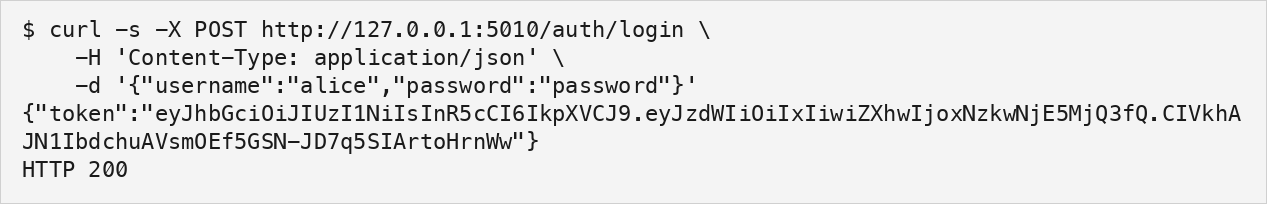
\includegraphics[width=\linewidth]{contents/demo-login.png}\\[0.6em]
Рисунок 1 --- Вход и выдача JWT
\end{center}

\begin{center}
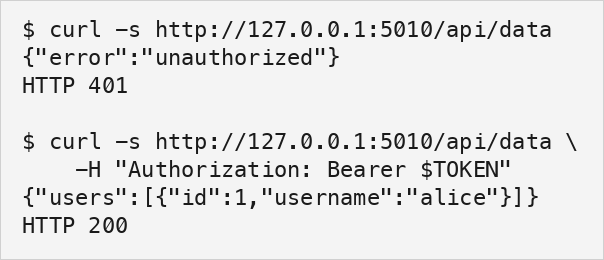
\includegraphics[width=\linewidth]{contents/demo-data.png}\\[0.6em]
Рисунок 2 --- Без токена доступ запрещён, с валидным токеном возвращается список пользователей
\end{center}

\begin{center}
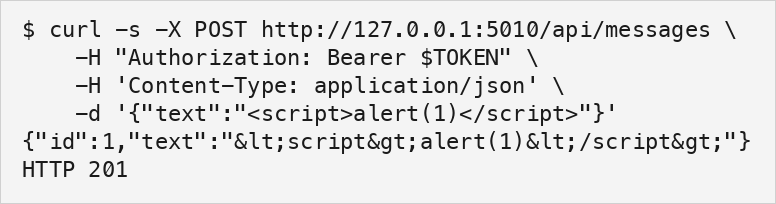
\includegraphics[width=\linewidth]{contents/demo-xss.png}\\[0.6em]
Рисунок 3 --- Защита от XSS: переданные теги возвращаются экранированными
\end{center}

\begin{center}
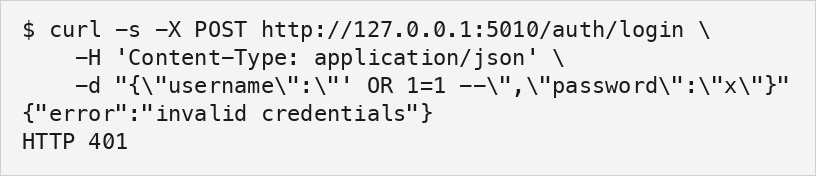
\includegraphics[width=\linewidth]{contents/demo-sqli.png}\\[0.6em]
Рисунок 4 --- Защита от SQL-инъекций: попытка обойти вход через инъекцию отклонена (401)
\end{center}

\head{Отчёты из pipeline}

На каждый push в ветку develop и при создании pull request в develop GitHub Actions запускает workflow: тесты (pytest), статический анализ кода bandit (SAST) и проверку зависимостей pip-audit (SCA). Все проверки проходят успешно.

\begin{center}
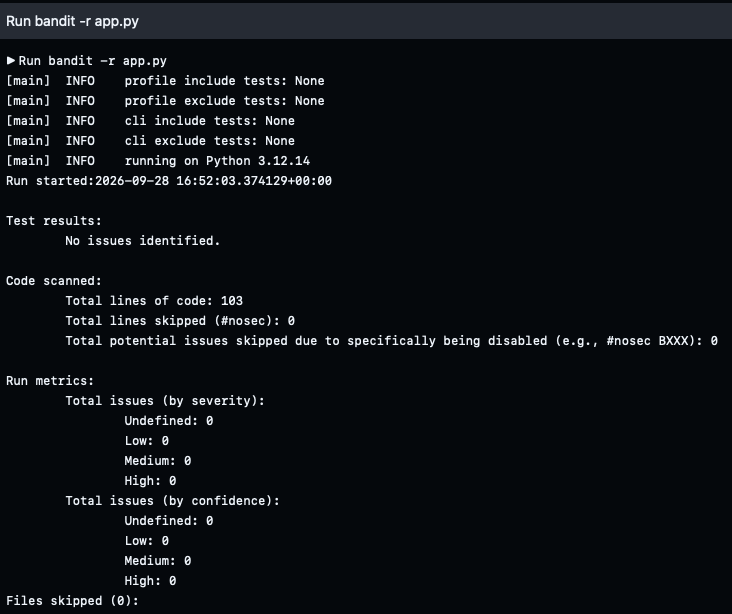
\includegraphics[width=\linewidth]{contents/sast.png}\\[0.6em]
Рисунок 5 --- Лог шага SAST (bandit): «No issues identified», High: 0
\end{center}

\begin{center}
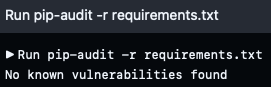
\includegraphics[width=0.62\linewidth]{contents/sca.png}\\[0.6em]
Рисунок 6 --- Лог шага SCA (pip-audit): «No known vulnerabilities found»
\end{center}

\head{Последний успешный запуск pipeline}

\url{https://github.com/tinunadno/ib-lab1/actions/runs/36454082460}

\end{document}
